\documentclass[10pt,a4paper]{article}
\usepackage{hyperref}
\usepackage{listings}
\usepackage[cm]{fullpage}
\usepackage{graphicx}


\title{IDAPI Coursework 2 - HepatitisC data set}
\author{Sebastian Grubb \href{mailto:sg3510@ic.ac.uk}{sg3510@ic.ac.uk}}
\date{\today}



\begin{document}
\maketitle


\section{Results}
\begin{verbatim}
Dependency Matrix
[[  0.00e+00   4.46e-02   2.57e-02   4.80e-02   3.40e-02   2.37e-02    3.91e-02   8.61e-02   1.57e-02]
 [  4.46e-02   0.00e+00   9.39e-03   6.04e-02   6.88e-02   3.03e-02    7.14e-02   8.26e-02   2.66e-03]
 [  2.57e-02   9.39e-03   0.00e+00   1.17e-02   7.15e-03   1.56e-03    7.02e-03   4.91e-03   5.18e-04]
 [  4.80e-02   6.04e-02   1.17e-02   0.00e+00   5.39e-01   2.75e-01    3.16e-02   3.24e-02   5.77e-03]
 [  3.40e-02   6.88e-02   7.15e-03   5.39e-01   0.00e+00   6.06e-01    4.06e-02   5.05e-02   8.40e-03]
 [  2.37e-02   3.03e-02   1.56e-03   2.75e-01   6.06e-01   0.00e+00    2.51e-02   4.14e-02   1.61e-02]
 [  3.91e-02   7.14e-02   7.02e-03   3.16e-02   4.06e-02   2.51e-02    0.00e+00   6.29e-02   3.85e-03]
 [  8.61e-02   8.26e-02   4.91e-03   3.24e-02   5.05e-02   4.14e-02    6.29e-02   0.00e+00   3.20e-02]
 [  1.57e-02   2.66e-03   5.18e-04   5.77e-03   8.40e-03   1.61e-02    3.85e-03   3.20e-02   0.00e+00]]
 \end{verbatim}
 Note that the diagonal is set to 0 intentionally as this facilitates all calculations and is consistent with $D(p||p)=0$ \footnote{\url{http://www.cs.princeton.edu/courses/archive/fall11/cos597D/L03.pdf}}.
 
 \begin{verbatim}
 Dependency List
 [[  6.06e-01   4   5]
  [  5.39e-01   3   4]
  [  2.75e-01   3   5]
  [  8.61e-02   0   7]
  [  8.26e-02   1   7]
  [  7.14e-02   1   6]
  [  6.88e-02   1   4]
  [  6.29e-02   6   7]
  [  6.04e-02   1   3]
  [  5.05e-02   4   7]
  [  4.80e-02   0   3]
  [  4.46e-02   0   1]
  [  4.14e-02   5   7]
  [  4.06e-02   4   6]
  [  3.91e-02   0   6]
  [  3.40e-02   0   4]
  [  3.24e-02   3   7]
  [  3.20e-02   7   8]
  [  3.16e-02   3   6]
  [  3.03e-02   1   5]
  [  2.57e-02   0   2]
  [  2.51e-02   5   6]
  [  2.37e-02   0   5]
  [  1.61e-02   5   8]
  [  1.57e-02   0   8]
  [  1.17e-02   2   3]
  [  9.39e-03   1   2]
  [  8.40e-03   4   8]
  [  7.15e-03   2   4]
  [  7.02e-03   2   6]
  [  5.77e-03   3   8]
  [  4.91e-03   2   7]
  [  3.85e-03   6   8]
  [  2.66e-03   1   8]
  [  1.56e-03   2   5]
  [  5.18e-04   2   8]]
 Spanning Tree
 [[ 0.61  4  5]
  [ 0.54  3  4]
  [ 0.09  0  7]
  [ 0.08  1  7]
  [ 0.07  1  6]
  [ 0.07  1  4]
  [ 0.03  7  8]
  [ 0.03  0  2]]
\end{verbatim}
\section{Graph}
\begin{figure}[h!]
  \caption{Graph of Hepatitis C dependency}
  \centering
    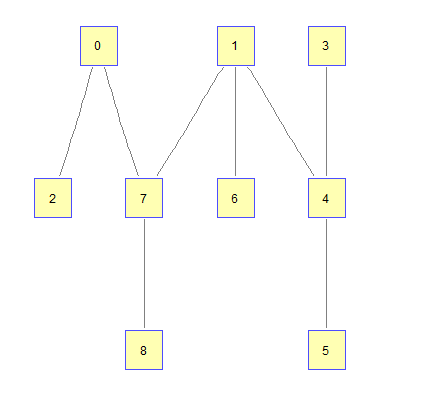
\includegraphics[width=0.5\textwidth]{network.png}
\end{figure}
Nodes on top are not necessarily meant to be root nodes this is simply the way \texttt{matlab}'s biograph function outputs the graph.
\section{Dependency Matrix with diagonal}
\begin{verbatim}
Dependency Matrix
[[  1.53e+00   4.46e-02   2.57e-02   4.80e-02   3.40e-02   2.37e-02    3.91e-02   8.61e-02   1.57e-02]
 [  4.46e-02   2.37e+00   9.39e-03   6.04e-02   6.88e-02   3.03e-02    7.14e-02   8.26e-02   2.66e-03]
 [  2.57e-02   9.39e-03   9.92e-01   1.17e-02   7.15e-03   1.56e-03    7.02e-03   4.91e-03   5.18e-04]
 [  4.80e-02   6.04e-02   1.17e-02   1.70e+00   5.39e-01   2.75e-01    3.16e-02   3.24e-02   5.77e-03]
 [  3.40e-02   6.88e-02   7.15e-03   5.39e-01   2.41e+00   6.06e-01    4.06e-02   5.05e-02   8.40e-03]
 [  2.37e-02   3.03e-02   1.56e-03   2.75e-01   6.06e-01   1.83e+00    2.51e-02   4.14e-02   1.61e-02]
 [  3.91e-02   7.14e-02   7.02e-03   3.16e-02   4.06e-02   2.51e-02    2.63e+00   6.29e-02   3.85e-03]
 [  8.61e-02   8.26e-02   4.91e-03   3.24e-02   5.05e-02   4.14e-02    6.29e-02   1.49e+00   3.20e-02]
 [  1.57e-02   2.66e-03   5.18e-04   5.77e-03   8.40e-03   1.61e-02    3.85e-03   3.20e-02   7.54e-01]]
\end{verbatim}

\end{document}